% SE-801 Term Project, Track S1, internal draft report
% Format: IEEE two-column conference (IEEEtran), as the protocol requires.
\documentclass[conference]{IEEEtran}

\usepackage{amsmath,amssymb}
\usepackage{graphicx}
\usepackage{booktabs}
\usepackage{multirow}
\usepackage{xcolor}
\usepackage{tikz}
\usetikzlibrary{arrows.meta,positioning,fit,calc}
\usepackage{pgfplots}
\pgfplotsset{compat=1.17}
\usepackage[hidelinks]{hyperref}
\usepackage{cite}

% Anything still waiting on the Atlas run or a pending re-run is marked in red.
\newcommand{\pending}[1]{\textcolor{red}{[#1]}}
\newcommand{\pmv}[2]{#1\,$\pm$\,#2}
\newcommand{\feat}[1]{\texttt{\detokenize{#1}}}

\begin{document}

\title{Physics-Guided Micro-Doppler Descriptors with Classical Learners, an MLP and Verified LLM Reporting for Small Aerial Target Classification\\
\large SE-801 Term Project, Track S1 (Internal Draft, 19 September 2026)}

\author{\IEEEauthorblockN{\pending{Student name}, Track S1}
\IEEEauthorblockA{SE-801 Artificial Neural Networks, Spring 2026\\
Supervisors: Dr Raja Farrukh Ali, Dr Salman Liaquat; dataset contact: Shaiq-e-Mustafa}}

\maketitle

\begin{abstract}
We ask whether a small multilayer perceptron (MLP) can learn more useful nonlinear combinations of ten physics-guided micro-Doppler descriptors than an RBF support vector machine (SVM), a Random Forest (RF) and XGBoost, using 75,801 complex I/Q segments from 130 measurements of a 77\,GHz FMCW radar in four classes (drone, bird, human, corner reflector) under a frozen nested 5$\times$5 cross-validation whose folds are disjoint by measurement. The SVM reaches a macro-F1 of \pmv{0.8771}{0.0248}, ahead of XGBoost (0.8625), Random Forest (0.8353) and the MLP (0.8294), against a majority baseline of 0.2183. The MLP is therefore the weakest of the four, not merely no better. The most accurate model is not the most trustworthy: Random Forest has the lowest calibration error, XGBoost the lowest Brier score and by far the best high-confidence operating point, while the SVM has the most confident errors and the MLP the worst Brier score. Under additive noise all models collapse, and for the two tree models intermediate noise (0\,dB) is worse than total noise, dropping them below the majority baseline because shifted features produce confident errors; the SVM and the MLP never cross it. The drone class splits into translating and hovering sub-populations that fail in opposite directions. For verified LLM reporting, a deterministic claim checker shows that numerical fabrication is rare and that almost all failures are ranking errors, and the checker itself needed validation: six of seven bugs found in it each changed a reported rate. Batch-one inference costs 0.023\,ms (MLP, CPU), 0.145\,ms (XGBoost), 0.388\,ms (SVM) and 10.235\,ms (Random Forest), so accuracy and serving cost are almost exactly reversed. The three classical models reproduce exactly across two machines while the MLP does not, making fixed-seed reproducibility a property of a device rather than of a configuration.
\end{abstract}

\begin{IEEEkeywords}
micro-Doppler, FMCW radar, drone classification, physics-guided features, calibration, robustness, LLM verification
\end{IEEEkeywords}

\section{Introduction}
Small drones, birds and people can appear alike to a surveillance radar: all are slow, small and close to the ground. Their micro-Doppler signatures, the frequency modulation produced by rotating blades, flapping wings and swinging limbs, are what separate them. The SE-801 project compares four families of models on one shared data package, protocol and metric set. Track S1 owns the physics-guided branch: ten handcrafted descriptors, three classical learners, a PyTorch MLP on the same descriptors, and a mandatory study of whether a large language model (LLM) can summarise the resulting numbers without inventing or misreporting them.

The principal S1 question is whether an MLP learns useful nonlinear combinations of the descriptors that conventional classifiers cannot (RQ3). S1 also contributes the classical reference for RQ2, the feature-based part of RQ10, and the answers to RQ8 (robustness), RQ9 (accuracy versus trust) and RQ11 (LLM reporting). Following the project instruction that the aim is not the highest accuracy, this report tries to state what was learned, why it works, when it fails, how reliable it is and what it costs.

Contributions to date:
\begin{itemize}
\item A leakage-free evaluation on real FMCW I/Q data, with folds grouped by measurement and frozen by hash, after the originally specified image dataset was found to leak between neighbouring frames.
\item Ten descriptors implemented from the signal rather than from images, with seven corrections to an earlier draft that each changed feature values silently.
\item A full four-model comparison with calibration, confidence, ablation, importance, data-efficiency and robustness analyses.
\item Evidence that the drone class holds two physically distinct sub-populations, and that reflector recall depends on range.
\item A deterministic LLM claim verifier, and a catalogue of seven verifier bugs, six of which would each have produced a wrong conclusion.
\end{itemize}
This is a working draft. Every radar result in this report comes from Atlas: job 2305 for the four models, latency and memory, job 2308 for the MLP inference latency and job 2309 for the ablations, data efficiency, importance and robustness. Only the LLM study was run locally, since it needs no cluster. The local development run agrees with Atlas to four decimal places everywhere except the MLP (Section~\ref{sec:compute}). Items still waiting are marked \pending{in red}.

\section{Radar and Stochastic Background}
\subsection{Micro-Doppler and the two axes}
A scatterer with radial velocity $v_r$ shifts the carrier by $f_D = 2v_r/\lambda$. At 77\,GHz, $\lambda \approx 3.9$\,mm. Parts of a target that move relative to its body add time-varying shifts on top of the bulk Doppler; this is micro-Doppler~\cite{chen2006}. Rotor blades turn at tens of revolutions per second with tip speeds of 69 to 92\,m/s here, so they produce short, wide-band blade flashes that repeat at the blade rate. Bird wings flap at a few hertz with far lower speeds, producing slow, narrow oscillations about the body line. In a segment, the slow-time axis (pulse to pulse) is the time axis; its Fourier transform gives the Doppler axis, which is radial velocity. The zero-Doppler region holds returns from stationary or near-stationary scatterers: clutter, a corner reflector, a hovering drone's body.

\subsection{Resolution and aliasing}
The radar samples slow time at a PRF of 17\,kHz, so the unambiguous velocity is $\pm\lambda\,\mathrm{PRF}/4 \approx \pm16.55$\,m/s. Rotor tips fold several times around this interval. Shaiq-e-Mustafa's guidance was to treat this aliasing as part of the signature rather than a defect, since the folded energy still separates rotors from wings. A 256-sample segment lasts 15\,ms and gives a Doppler bin of 66.4\,Hz, or 0.13\,m/s. The short-time Fourier transform (STFT) used for the temporal descriptors trades these off: a 64-sample window (3.8\,ms) gives 13 frames with 75\% overlap but a coarser bin of 0.52\,m/s. A 15\,ms dwell covers one or two rotor revolutions but only a small fraction of a wing beat, which later explains why the temporal descriptors carry little information.

\subsection{Why this matters for the protocol}
Flipping or shifting a spectrogram is not a harmless augmentation: a flip swaps approaching and receding motion and a shift changes velocity. Images also discard the phase and absolute power that raw I/Q keeps. Corrupting I/Q with noise is a physical-signal perturbation, while blurring a computed spectrum is representation-domain, and we keep that distinction throughout (Section~\ref{sec:robust}).

\subsection{Stochastic elements}
\label{sec:stoch}
Added noise is circularly symmetric complex Gaussian, $n \sim \mathcal{CN}(0,\sigma_n^2)$ with $\mathbb{E}[n]=0$ and $\mathrm{Var}[n]=\sigma_n^2 = P_s/10^{s/10}$, where $P_s$ is the mean power of the segment and $s$ the target SNR in dB. The variance is split equally between the real and imaginary parts. For pure noise, each periodogram bin is exponentially distributed, so its standard deviation equals its mean; a noisy spectrum therefore looks flat on average and jagged in any single draw, which drives entropy up and makes moment features unstable. Each segment draws its noise from a generator seeded by a hash of its identifier and the condition name, so every model sees exactly the same corrupted sample. Preprocessing is deterministic; no stochastic augmentation is used. Fold-level mean and standard deviation describe variability over which measurements land in the test fold, not over repeated draws of a fixed test set: with five outer folds, a standard deviation of 0.025 means the ranking of models closer than about that amount is not established. All classifiers output class probabilities, which Section~\ref{sec:calib} evaluates as probabilities rather than as labels.

\section{Dataset and Deviations from the Protocol}
\subsection{Why the dataset changed}
The specification fixes DIAT-$\mu$SAT~\cite{kumawat2022}. Before the freeze, Syed Zain Ul Hassan measured the similarity between images in each class folder: consecutive frames scored 0.94 to 0.99 against 0.68 to 0.85 for distant frames, showing that the images are overlapping frames of continuous recordings. Any random split would put near-copies on both sides. Dr Salman Liaquat approved a move to raw radar data.

\subsection{The Karlsson FMCW dataset}
We use the KTH dataset of Karlsson et al.~\cite{karlsson2022,karlsson_zenodo}, recorded with a SAAB SIRS~1600 77\,GHz FMCW radar (160\,MHz bandwidth, about 1\,m range resolution, PRF 17\,kHz). Each segment is 5 range cells by 256 slow-time samples. Shaiq-e-Mustafa mapped the fifteen raw labels to four coarse classes (Table~\ref{tab:data}). We drop the 67 segments flagged as field-of-view edge, leaving 75,801. The feature file holds all 75,868 rows and the exclusion is applied when the training table is loaded, which both runs report explicitly (\texttt{75868 -> 75801}), so the count cannot drift silently. The data are heavily imbalanced: drones are 77.5\% of segments, which is why macro-F1 is the primary metric.

\begin{table}[t]
\centering
\caption{Class mapping and sizes (after excluding 67 edge segments from 75,868).}
\label{tab:data}
\begin{tabular}{lrrl}
\toprule
Class & Meas. & Segments & Files \\
\midrule
Drone & 44 & 58,768 & 000 to 043 \\
Human & 11 & 6,028 & 044 to 054 \\
Bird & 56 & 7,792 & 055 to 110 \\
Corner reflector & 19 & 3,280 & 111 to 129 \\
\midrule
Total & 130 & 75,868 & \\
\bottomrule
\end{tabular}
\end{table}

A negative finding about the source: the authors' own train/validation/test indicator is not disjoint by measurement. Their published figures (78\% out-of-distribution accuracy rising to 86\% with a synthetic class, about 90\% overall, on 150 sweeps or 9\,ms) therefore share the leakage character that took the project off DIAT-$\mu$SAT, and are not directly comparable with ours.

\subsection{Documented deviations}
Table~\ref{tab:dev} lists every departure from the written specification and its reason. Each was approved by a supervisor or follows necessarily from an approved change.

\begin{table}[t]
\centering
\caption{Deviations from the written protocol.}
\label{tab:dev}
\footnotesize
\begin{tabular}{p{0.33\columnwidth}p{0.57\columnwidth}}
\toprule
Change & Reason \\
\midrule
DIAT-$\mu$SAT $\rightarrow$ Karlsson FMCW & Frame leakage; approved by Dr Salman \\
Six classes $\rightarrow$ four & Classes of the new data; set by Shaiq \\
Image pipeline $\rightarrow$ I/Q DSP & Grayscale, crop and min-max have no meaning for complex data \\
Intensity noise $\rightarrow$ complex I/Q noise & Physical-signal noise is now possible; blur stays representation-domain \\
Zero-Doppler band $\pm$0.075 & ``Central 15\%'' has two readings; chosen by sweep (Sec.~\ref{sec:zd}) \\
Main-lobe half-width 0.10 & Not specified by the protocol \\
67 edge segments dropped & Flagged by the dataset authors \\
Signed log on moments & Heavy tails; applied before fold-scoped scaling \\
Grouped SVM calibration & SVC's internal Platt step is not group-aware \\
MLP output 4, not 6 & Follows the class change \\
\bottomrule
\end{tabular}
\end{table}

\section{Methodology and Process Workflow}
\subsection{Workflow}
Fig.~\ref{fig:pipeline} shows the pipeline. It ran in this order, and each stage writes a machine-readable artifact that the next reads: (1) freeze the dataset and fold manifests; (2) convert I/Q to normalised power and store it as a memory map; (3) extract the ten descriptors; (4) validate them numerically and choose the zero-Doppler band by sweep; (5) nested cross-validation of the three classical models, saving out-of-fold probabilities and fitted models; (6) the MLP with the same folds; (7) error analysis and model comparison; (8) ablations, importance and data efficiency; (9) robustness; (10) the LLM reporting study. Every formal run appends a row to a shared run ledger. A checker script confirms that all seventeen scripts are the current revision before any run whose numbers reach this report; a stale verifier once produced two false failure rates that were nearly reported.

\begin{figure*}[t]
\centering
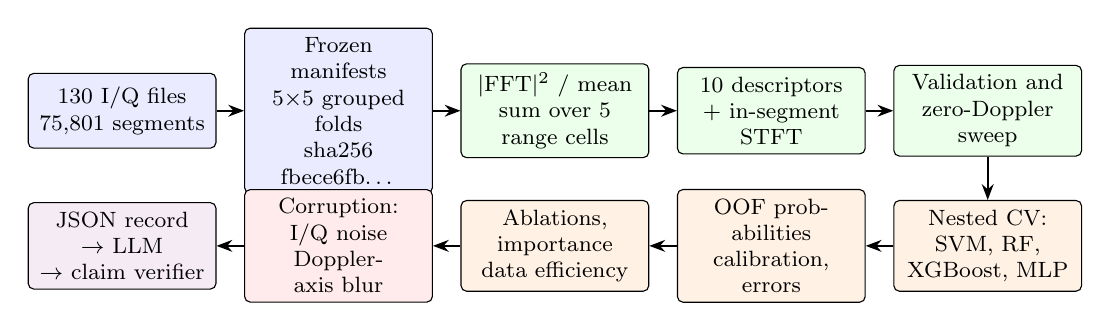
\begin{tikzpicture}[
  box/.style={draw, rounded corners=2pt, align=center, font=\footnotesize, minimum height=0.95cm, text width=2.15cm, fill=#1},
  box/.default=white,
  arr/.style={-{Stealth[length=2mm]}, thick}]
\node[box=blue!8] (a) {130 I/Q files\\75,801 segments};
\node[box=blue!8, right=0.35cm of a] (b) {Frozen manifests\\5$\times$5 grouped folds\\sha256 fbece6fb\ldots};
\node[box=green!8, right=0.35cm of b] (c) {$|\mathrm{FFT}|^2$ / mean\\sum over 5 range cells};
\node[box=green!8, right=0.35cm of c] (d) {10 descriptors\\+ in-segment STFT};
\node[box=green!8, right=0.35cm of d] (e) {Validation and\\zero-Doppler sweep};
\node[box=orange!10, below=0.55cm of e] (f) {Nested CV:\\SVM, RF,\\XGBoost, MLP};
\node[box=orange!10, left=0.35cm of f] (g) {OOF probabilities\\calibration, errors};
\node[box=orange!10, left=0.35cm of g] (h) {Ablations, importance\\data efficiency};
\node[box=red!8, left=0.35cm of h] (i) {Corruption: I/Q noise\\Doppler-axis blur};
\node[box=violet!8, left=0.35cm of i] (j) {JSON record $\rightarrow$ LLM\\$\rightarrow$ claim verifier};
\draw[arr] (a)--(b); \draw[arr] (b)--(c); \draw[arr] (c)--(d); \draw[arr] (d)--(e);
\draw[arr] (e)--(f); \draw[arr] (f)--(g); \draw[arr] (g)--(h); \draw[arr] (h)--(i); \draw[arr] (i)--(j);
\end{tikzpicture}
\caption{S1 process workflow. Blue: frozen data and folds. Green: signal processing and features. Orange: learning and analysis. Red: robustness. Violet: LLM reporting. Each box writes a stored artifact that the next box reads, so every table can be regenerated from files.}
\label{fig:pipeline}
\end{figure*}

\subsection{Signal processing}
For each segment the slow-time FFT is taken per range cell and converted to power $|X|^2$, divided by its own mean so that absolute return level cannot act as a range proxy. We use linear power: no logarithm, no min-max scaling and no ``pseudo-power'' from squared image intensities, all of which came from the image protocol and, as found in an earlier draft, destroyed the power relationships. The five range cells are summed, giving the total power at each Doppler bin across the target's extent. We deliberately do not re-centre the spectrum on the bulk Doppler, so that the zero-Doppler descriptor remains a real test of whether a target is stationary.

\subsection{The ten descriptors}
With $p_k$ the normalised Doppler power at normalised frequency $f_k \in [-1,1)$: \emph{Doppler spread} is the power-weighted standard deviation $\sigma$; \emph{skewness} and \emph{kurtosis} are power-weighted third and fourth standardised moments (excess kurtosis); \emph{80\% bandwidth} is the width between the 10th and 90th percentiles of the Doppler CDF; \emph{spectral entropy} is $-\sum p_k\ln p_k/\ln K$; the \emph{zero-Doppler ratio} is the mass with $|f_k|\le 0.075$; the \emph{side-lobe energy ratio} is the mass outside $\pm0.10$ of the dominant peak, and \emph{side-lobe entropy} is the normalised entropy of that mass. From the in-segment STFT (64-sample Hann window, 48 overlap, 13 frames), \emph{temporal energy variance} is the squared coefficient of variation of frame energy and \emph{temporal entropy} is the normalised entropy of frame energy.

Seven corrections to an inherited draft each changed values without raising an error: unweighted skewness was blind to the sign of Doppler asymmetry; the old bandwidth grew a window about zero and so measured speed rather than width; a side-lobe ratio defined about zero Doppler was exactly one minus the zero-Doppler ratio (correlation $-1.000$); a library spectrogram removed the mean of each window, erasing stationary targets, and then squared power a second time; temporal variance was made scale-free; entropies were normalised; the Doppler axis was normalised. Skewness and kurtosis receive a signed $\log(1+|x|)$ before a StandardScaler that is fitted on the training fold only.

\subsection{Zero-Doppler band}
\label{sec:zd}
``The central 15\% of the Doppler axis'' can mean $\pm0.15$ (77 bins, $\pm$2.48\,m/s) or $\pm0.075$ (19 bins, $\pm$1.24\,m/s). A walking person moves at about 1.4\,m/s and falls inside the wider band. A sweep settled the choice: the rank AUC separating drones from humans on this descriptor is 0.814 at 0.075 and 0.412 at 0.150, the latter being worse than chance. We froze 0.075.

\subsection{Evaluation protocol}
Folds come from StratifiedGroupKFold grouped by measurement, five outer folds (seeds 2026 to 2030) and five inner folds, frozen in a write-once manifest (sha256 \texttt{fbece6fb\ldots a8d9e8468c}) that every track shares. Hyperparameters are chosen by mean inner-fold macro-F1 over the mandated grids: SVM $C\in\{1,10,100\}$, $\gamma\in\{\text{scale},0.01,0.1\}$; RF with 500 trees, depth $\in\{\text{None},10,20\}$, leaf $\in\{1,3\}$; XGBoost trees $\in\{200,500\}$, depth $\in\{3,6\}$, rate $\in\{0.03,0.1\}$. Outer-test folds are never used for selection, calibration or tuning. We report the mean and standard deviation over the five outer folds, never the best fold.

\subsection{MLP and the training loop}
The MLP is 10$\rightarrow$64$\rightarrow$32$\rightarrow$4 with ReLU, batch normalisation and dropout 0.3 (3,108 parameters), trained with AdamW, batch 64, unweighted cross-entropy, gradient clipping at 1.0, up to 60 epochs and early stopping with patience 8, over the grid lr $\in\{10^{-4},3\cdot10^{-4},10^{-3}\}$ and weight decay $\in\{10^{-5},10^{-4}\}$. The loop follows the ten protocol steps (loading, gradient reset, forward, loss, backward, update, validation, early stopping, checkpoint save and restore) and logs loss and macro-F1 for both splits, gradient norms and epoch time. \texttt{model.train()} enables dropout and batch statistics; \texttt{model.eval()} disables dropout and uses running statistics, so a test prediction cannot depend on the other samples in its batch. A small-batch overfitting test and a fixed-seed repeat are built in; a first version of the repeat drew the first 4,000 rows, all one class, and returned a meaningless 0.2500, so it now samples by class and refuses degenerate subsets. On Atlas the fixed-seed test passed on a balanced 8,000-row subset: two runs of seed 2026 gave identical per-epoch loss curves, an identical best validation macro-F1 of 0.81052 at epoch 24, and identical predicted probabilities. The small-batch test passed cleanly on Atlas: 32 samples balanced across the four classes, driven to training loss 0.0416 with accuracy and macro-F1 both 1.000 in 400 epochs, which rules out broken gradient flow, mislabelled inputs and an unusable learning rate as explanations for the network's modest full-data score.

\subsection{Calibration and confidence}
\label{sec:calib}
For each outer-test segment we store the full probability vector and compute top-1 and top-2 accuracy, maximum confidence, prediction entropy, coverage and accuracy above confidence thresholds, the rate of confident errors, ECE with 15 equal-width bins, Brier score and reliability diagrams. The SVM's built-in Platt scaling uses a random internal split, which is not grouped by measurement and leaks optimistic scores into calibration. We instead wrap the SVM in a sigmoid \texttt{CalibratedClassifierCV} with explicit grouped splits of the training fold.

\subsection{Robustness}
\label{sec:robust}
Conditions follow the protocol levels: complex I/Q noise at $-10$, $-5$, 0, $+5$ and $+10$\,dB (Section~\ref{sec:stoch}), Doppler-axis Gaussian blur of the power spectrum at $\sigma=1,2,4$ bins, and a combined 0\,dB plus 2-bin condition. The noise is a physical-signal perturbation added to the recorded samples, and because that reference power already contains receiver noise, ``0\,dB'' means added noise equal to the recorded segment power rather than a true target SNR. The blur acts on a computed spectrum, so it is a representation-domain surrogate for phase instability, never physical phase noise. Corruption is applied after fold splitting, to test data only, models are not retuned, and every feature is recomputed from the corrupted signal; a first version fed clean I/Q to the temporal descriptors, which showed up as a rank correlation of exactly 1.000.

\subsection{LLM reporting study}
A record of 50 numeric facts (fold scores, means, standard deviations, accuracy, ECE, Brier and more) is built from the stored results. Four arms are compared: direct prompting with the raw JSON, constrained prompting that demands source values only, generate-and-verify in which a failing summary is returned once with the verifier's report for correction, and a verifier-validation arm with seeded errors. The verifier is deterministic Python, not an LLM judge. It labels every number as supported, derived, altered, unsupported or echoed from the prompt, and checks every superlative and pairwise comparison at clause level against the record, marking claims it cannot bind as unchecked rather than guessing. We report numerical factual accuracy, unsupported-claim rate, pass rate with Wilson 95\% intervals, numbers per summary and coverage (the fraction of the record reported). Models: Gemini 3.5 Flash, Llama 3.1 8B and Llama 3.2 3B (local, via Ollama).

\subsection{Compute and cross-machine reproduction}
\label{sec:compute}
Every radar number comes from Atlas; the local machine, an Intel i9-12900 (24 threads, 32\,GB) with an RTX A4000, served only as the development environment. The final run uses one Atlas Argon node (\texttt{argon01}, RTX 4090) in a single allocation that stages the data to node-local scratch, recomputes features and re-runs training, calibration, the MLP demonstrations and latency (100 warm-up and 1,000 timed batch-one inferences, repeated five times and averaged, as Dr Farrukh advised). The Atlas stack has scikit-learn 1.8.0 against 1.9 locally, so small numerical differences were expected; there are none. The Atlas run recomputes every descriptor from the staged I/Q and returns the same majority baseline (\pmv{0.2183}{0.0007}) and the same macro-F1, accuracy, ECE and Brier score as the local run for all three classical models, agreeing to four decimal places on every outer fold (SVM 0.8306, 0.8822, 0.9036, 0.8904, 0.8786). Because the fold manifest is shared rather than regenerated, this is an end-to-end check of the signal processing and feature code across two operating systems, two BLAS builds and two library versions, not only of the split.

The MLP behaves differently, and the contrast deserves stating rather than smoothing over. Trained on the GPU it returns \pmv{0.8294}{0.0319} against \pmv{0.8338}{0.0305} on the local CPU, with per-fold differences of $-0.011$ to $+0.001$ and ECE and Brier moving by about 0.005. The deviation sits well inside the fold standard deviation and changes no conclusion, but it is not zero, whereas the classical models differ by nothing at all. Within one device the network is exactly reproducible: the fixed-seed test on Atlas gave identical loss curves and identical predicted probabilities across two runs of seed 2026 on a balanced 8,000-row subset. Across devices it is not. Two causes are present and one run each cannot separate them: the reduction order of floating-point accumulation differs between CPU and CUDA kernels, and the two machines also run different PyTorch versions (2.13.0 locally, 2.5.1 on Atlas). Either is enough to move the last bits of a gradient, and a 42-epoch trajectory amplifies the difference. Seeding makes a run repeatable on the machine that ran it and nothing more; portable reproducibility belongs to the deterministic parts of the pipeline. 

\section{Results}
\subsection{Model comparison (RQ2, RQ3)}
Table~\ref{tab:main} gives the headline results. All four models are far above the majority baseline. The SVM leads on macro-F1 and accuracy, and its margin over XGBoost (0.015) is smaller than either model's fold standard deviation, so their order is suggestive rather than established. On Atlas the MLP is last rather than tied: 0.8294, which is 0.0059 below Random Forest and 0.048 below the SVM, and it is the only model whose score depends on which machine ran it. It is also the most expensive to train on equal hardware, 49\,m 48\,s on the RTX 4090 against 9\,m 09\,s for the SVM and 1\,m 30\,s for XGBoost on the same node.

\begin{table}[t]
\centering
\caption{Clean accuracy and calibration, mean $\pm$ s.d. over five outer folds. Generated from the stored results by \texttt{compare\_models.py}.}
\label{tab:main}
\footnotesize
\setlength{\tabcolsep}{4pt}
\begin{tabular}{lccccc}
\toprule
Model & Macro-F1 & Acc. & ECE & Brier & Top-2 \\
\midrule
Majority baseline & .2183 $\pm$ .0007 &  &  &  &  \\
RBF-SVM & \textbf{.8771} $\pm$ .0248 & \textbf{.9379} & .0281 & .1108 & \textbf{.9891} \\
XGBoost & .8625 $\pm$ .0369 & .9300 & .0258 & \textbf{.1091} & .9853 \\
Random Forest & .8353 $\pm$ .0396 & .9181 & \textbf{.0213} & .1249 & .9824 \\
MLP & .8294 $\pm$ .0319 & .9106 & .0260 & .1332 & .9860 \\
\bottomrule
\end{tabular}
\end{table}


\begin{table}[t]
\centering
\caption{Computational cost, Section 18 items. Batch-one latency on one Argon node, 100 warm-up and 1,000 timed inferences, five repeats. Generated from the stored results by \texttt{compare\_models.py}.}
\label{tab:cost}
\footnotesize
\setlength{\tabcolsep}{2.5pt}
\begin{tabular}{@{}llrrrr@{}}
\toprule
Model & Size & Lat. & p95 & Spread & Train \\
 & & (ms) & (ms) & (ms) & (min) \\
\midrule
MLP, CPU & 3108 weights & \textbf{.023} & .024 & .0002 & 49.8 \\
MLP, CUDA & 3108 weights & .056 & .057 & .0005 & 49.8 \\
XGBoost & 500 trees, depth 6 & .145 & .153 & .0015 & \textbf{1.5} \\
RBF-SVM & 7,333 SVs & .388 & .402 & .0028 & 9.2 \\
Random Forest & 500 trees, no cap & 10.235 & 10.423 & .0441 & 21.1 \\
\bottomrule
\end{tabular}
\end{table}


Table~\ref{tab:fold} shows that the SVM wins on every class, not only on the average, and that fold 0 is the hardest for every model. Per-class F1 there is pooled over all out-of-fold predictions, which hides how unevenly the classes behave across folds: the human class varies by 0.088 to 0.118 between folds while drones vary by 0.009 to 0.011. Model selection was stable: the SVM chose $C=100$, $\gamma=$ scale in all folds; XGBoost chose rate 0.1, depth 6, 500 trees in all folds; RF chose unlimited depth and leaf 1 (leaf 3 in fold 0); the MLP chose lr $10^{-3}$ in every fold, with weight decay $10^{-4}$ in folds 0 and 2 and $10^{-5}$ in the others. Every selection except that weight decay lies on the edge of its grid, a limitation we return to below. The MLP stopped early in all five folds (18 to 44 epochs run, best epoch 9 to 35), so the 60-epoch budget was never the binding constraint.

\begin{table}[t]
\centering
\caption{Per-fold macro-F1 and pooled per-class F1. Generated from the stored results by \texttt{compare\_models.py}.}
\label{tab:fold}
\footnotesize
\setlength{\tabcolsep}{3pt}
\begin{tabular}{lccccc|cccc}
\toprule
& \multicolumn{5}{c|}{Outer fold} & \multicolumn{4}{c}{Class F1} \\
Model & 0 & 1 & 2 & 3 & 4 & Dro. & Bird & Hum. & Refl. \\
\midrule
RBF-SVM & .831 & .882 & .904 & .890 & .879 & .969 & .792 & .833 & .920 \\
XGBoost & .797 & .903 & .867 & .890 & .856 & .964 & .780 & .818 & .888 \\
Random Forest & .761 & .861 & .832 & .874 & .850 & .955 & .752 & .797 & .842 \\
MLP & .770 & .864 & .827 & .842 & .844 & .951 & .710 & .801 & .849 \\
\bottomrule
\end{tabular}
\end{table}


\begin{figure}[t]
\centering
\IfFileExists{figures/reliability.pdf}
  {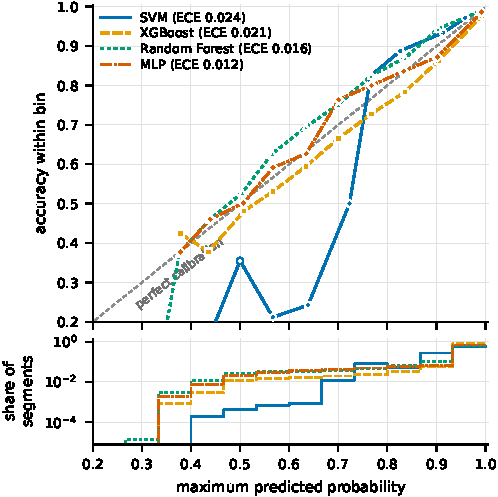
\includegraphics[width=0.92\columnwidth]{figures/reliability.pdf}}
  {\fbox{\parbox[c][3.4in][c]{0.92\columnwidth}{\centering\footnotesize
   \texttt{figures/reliability.pdf}\\ generated by \texttt{make\_reliability.py}}}}
\caption{Reliability over 15 equal-width confidence bins, pooled over all
out-of-fold predictions; the dashed diagonal is perfect calibration. Hollow
markers mark bins holding fewer than 50 segments. The lower panel gives each model's share of segments per bin on a log
scale, which is what separates the SVM from XGBoost at the right-hand edge:
both are near the diagonal there, but the SVM puts 3\% of its mass in that
region against XGBoost's 65\%. ECE values in the legend are pooled and
therefore differ from the fold-averaged values in Table~\ref{tab:main}.}
\label{fig:rel}
\end{figure}

\subsection{Cost, latency and measurement stability}
Table~\ref{tab:cost} answers the computational part of the project question, and one result was not obvious in advance. XGBoost is both the cheapest to train (1\,m 30\,s for the whole nested procedure) and the fastest at inference (0.145\,ms per segment), while Random Forest, with the same number of trees, is 70 times slower at 10.235\,ms because its selected configuration leaves depth uncapped and leaf size at one, so each tree is large. Depth, not tree count, sets the inference cost. The SVM sits between them at 0.388\,ms while storing an average of 7,333 support vectors, about 73,000 feature values, against the MLP's 3,108 parameters: the most accurate model is also the largest, yet still fast enough for a 15\,ms dwell by a factor of forty.

The MLP inverts the usual expectation twice. It is the cheapest model at inference, 0.023\,ms on the CPU, six times faster than XGBoost, because 3,108 weights are two small matrix products and nothing more. And it is 2.4 times \emph{slower} on the GPU than on the CPU, 0.056\,ms against 0.023\,ms, because at batch one the work is far smaller than the cost of launching kernels and synchronising; the accelerator that cut training from 112 to 50 minutes is a liability for single-sample inference. Both numbers are reported, and the CPU figure is the one comparable with the classical models. So the accuracy ordering and the inference-cost ordering are almost exactly reversed: the weakest model is the cheapest to serve and the most expensive to train.

Dr Farrukh's caution that latency measurement is unreliable on repetition is answered by the repeats rather than assumed. Five independent passes of the 100 warm-up and 1,000 timed protocol per fold agree to 0.0015\,ms for XGBoost, 0.0028\,ms for the SVM, 0.0441\,ms for Random Forest and 0.0005\,ms for the MLP, which is 1.0\% of the mean or better in every case and under 0.9\% for the network on either device. The variation between folds (0.007, 0.010 and 0.152\,ms for the classical models) is larger than the variation between repeats. The worst single case is Random Forest in fold 4, where the repeat means drift from 10.23 to 10.07\,ms. So on a pinned Argon node the protocol is reproducible, and what little instability exists comes from the model being timed rather than from the timing.

Peak resident memory is 2.40, 2.38 and 2.31\,GB for the SVM, XGBoost and Random Forest, within 4\% of each other because the feature table and its fold copies dominate rather than the models, so on this track peak memory carries no information about method cost.

\subsection{Calibration and trust (RQ9)}
The ranking changes once probabilities are judged (Tables~\ref{tab:main} and~\ref{tab:conf}). Random Forest has the lowest ECE (0.0213) and XGBoost the lowest Brier score (0.1091), and the two do not agree because ECE asks whether confidence is right on average while Brier punishes individual errors. The most accurate model, the SVM, is fourth on ECE, and the MLP is last on Brier. XGBoost also offers by far the most useful high-confidence operating point: 65\% of segments receive $p\ge0.99$ with 98.9\% accuracy, against 3.5\% for the SVM. The SVM has the highest rate of confident errors. Its sigmoid calibration compresses probabilities away from 1, so it is rarely very sure and, when it is fairly sure, it is wrong more often than the others. Top-2 accuracy is 0.98 to 0.99 for every model, so the true class is almost always one of the two leading candidates. Confident errors are not spread evenly over the classes: of the SVM's 2,100 errors at $p\ge0.9$, 1,517 (72\%) assign a bird, human or reflector to the drone class, and the pattern repeats for every model. The majority class attracts the confident mistakes, which matters more operationally than the aggregate rate, since a missed bird called a drone is the alarm a counter-UAS system would act on. Fig.~\ref{fig:rel} gives the reliability diagrams, and they expose a choice the protocol leaves open. ECE fixes the bin count at 15 but not how folds are combined, and the two natural choices disagree: averaging the per-fold ECE gives 0.0281, 0.0258, 0.0213 and 0.0260 for SVM, XGBoost, Random Forest and MLP, while pooling every out-of-fold prediction into one set of bins gives 0.0241, 0.0212, 0.0157 and 0.0118. Both orderings agree that the SVM is the worst calibrated, but the MLP moves from third to first, because pooling lets miscalibration of opposite sign in different folds cancel and the MLP's per-fold ECE is the most variable of the four (0.014 to 0.059). We report the fold average in Table~\ref{tab:main} as the conservative figure and the pooled value in the figure, and note that a calibration claim should always say which one it means.

The shape of the curves adds one thing the numbers do not. Three of the four models lie above the diagonal over most of the confidence range, meaning they are conservative: they are right more often than they claim. The SVM is the only model that falls below the diagonal, between roughly 0.45 and 0.7 confidence, so it is the only one that is overconfident anywhere, which is consistent with its having the highest rate of confident errors. That dip sits in bins holding 45 segments in total out of 75,801, so it is a real direction on very little mass rather than a large effect, and the figure marks those points hollow for exactly that reason.

\begin{table}[t]
\centering
\caption{Confidence operating points on the pooled outer-test predictions of Atlas job 2305.}
\label{tab:conf}
\footnotesize
\begin{tabular}{lccc}
\toprule
Model & Coverage at $p\ge0.99$ & Acc. there & Wrong with $p\ge0.9$ \\
\midrule
SVM & 0.0347 & 99.66\% & 2.77\% \\
XGBoost & \textbf{0.6531} & 98.87\% & 2.35\% \\
RF & 0.4215 & 99.33\% & \textbf{1.06\%} \\
MLP & 0.5324 & 99.46\% & 1.40\% \\
\bottomrule
\end{tabular}
\end{table}

\subsection{Error analysis}
\emph{Drone sub-populations.} Splitting drone segments by zero-Doppler ratio quartile gives SVM recall 0.923, 0.980, 0.997 and 0.986 from lowest to highest. The lowest quartile holds translating drones, whose body line moves away from zero and which are confused with birds; the highest holds hovering drones, whose energy sits at zero Doppler and which are confused with the reflector or with humans. The class is internally split and its two tails fail for opposite physical reasons.

The feature-level evidence agrees. Median zero-Doppler ratios are 1.000 for the reflector, 0.848 for the drone class, 0.073 for birds and 0.068 for humans. The validation gate flags the reflector-to-drone margin of only 0.152, which is the hovering population showing up in the descriptor rather than a defect in the band: hovering drones genuinely are stationary targets by this measure.

\emph{Hard measurements.} Fold 0 is hardest for every model because it holds the running-human recordings 048, 050 and 054; a runner's body Doppler of about 3\,m/s resembles slow drones and birds. The single worst measurement is walking human 046 (per-model F1 0.17 to 0.32), whose speed of about 1.4\,m/s sits just outside the $\pm$1.24\,m/s zero-Doppler band, the band-edge case that motivated the sweep. Only three of 130 measurements (349 segments) defeat all four models: raven 068, pigeon 067 and walking human 046. The first two are the rare labels the dataset ReadMe flags.

\emph{Which class fails in which fold.} The confusion matrices localise the two weaknesses. Fold 0 is a human-class failure: SVM human F1 is 0.681 there against 0.821 to 0.896 elsewhere, and both tree models also send reflector segments to the human class (189 of 669 for RF, 95 for XGBoost). Folds 1 and 2 are reflector failures of the opposite kind, with 188 and 113 reflector segments called drone by the SVM, 206 and 300 by RF and 109 and 227 by XGBoost, while folds 3 and 4 make almost no such errors. Reflector and hovering drone are mutually confusable, and which direction the error takes depends on which recordings land in the test fold. With 19 reflector and 11 human measurements, a single recording moving between folds shifts a class F1 by a tenth.

\emph{Range confound, and how much of it is real.} Reflector recall against range is graded at the long end and should be read as a genuine effect: per-measurement SVM recall is 1.000 out to 100\,m, then 0.924 at 97\,m, 1.000 at 126\,m for one recording but 0.379 at 130\,m for another, and 0.626 at 172.6\,m, where Random Forest reaches 0.043 and the MLP 0.003. Falling SNR makes a distant spectrum noise-like, so part of what the classifier learns is range-dependent SNR rather than target physics.

The apparent weakness at close range is a different matter and we state it as a caveat rather than a trend. It rests on exactly two recordings, 112 at 9.4\,m and 113 at 15.1\,m, and every model scores them either 1.000 or 0.000: on 112 the SVM and the MLP are perfect while XGBoost and Random Forest score zero, and on 113 only Random Forest fails. Both sit in fold 0. That is a decision boundary falling on one side or the other of two short recordings, not a smooth degradation, and with 19 reflector measurements it would be wrong to report a close-range effect.

\emph{Failures that are not shared.} Consensus failures are rare, per-model failures are not. Besides the two reflector recordings above, measurement 003 (drone, 809 segments, fold 3) is recalled at 0.99 or better by all three classical models and at 0.577 by the MLP. So the MLP's deficit is not spread evenly over the data; it concentrates in places the classical models handle without difficulty.

\subsection{Features: ablation and importance (RQ10, S1 part)}
Table~\ref{tab:abl} summarises the ablations. Removing any single descriptor costs at most 0.026, and for three of ten features the SVM is very slightly better without them, so no descriptor is critical and the set is highly redundant. The spectral-shape family alone recovers 0.79 to 0.81, the energy family 0.73 and the two temporal descriptors only 0.29 to 0.41; dropping the temporal family costs at most 0.009. Neither informative family is sufficient or dispensable on its own: dropping spectral shape costs 0.057 to 0.102 and dropping energy distribution 0.045 to 0.055, while either alone loses more than either removal, which is what overlapping information looks like. This agrees with the physical argument in Section~II: a 15\,ms dwell cannot resolve wing-beat periodicity. The same three descriptors are the most important for every model, though not in the same order: the SVM ranks spectral entropy (0.464), Doppler spread (0.455) and side-lobe energy ratio (0.433), while XGBoost puts side-lobe energy ratio first (0.439) and Random Forest spectral entropy (0.249). Skewness and temporal energy variance are last for all three. The MLP weights the set differently: kurtosis is its second most important descriptor (0.368, against spectral entropy's 0.374), where XGBoost and Random Forest give kurtosis 0.074 and 0.034. A network with 3,108 weights can use a heavy-tailed shape descriptor that axis-aligned splits largely ignore, which is the one place where the MLP does something the trees do not. Large permutation importance alongside tiny leave-one-out deltas is the signature of redundancy: permuting one feature breaks the model that uses it, but retraining without it lets a correlated feature take over.

Five features are not enough either way, but how they are chosen matters. The subset picked from the correlation structure before any training (Doppler spread, temporal entropy, zero-Doppler ratio, side-lobe entropy, kurtosis) loses 0.053 to 0.086. The subset picked from permutation importance on the full-feature models (spectral entropy, Doppler spread, side-lobe energy ratio, kurtosis, zero-Doppler ratio) loses only 0.015 to 0.058, and it does so while deliberately taking three members of one correlated cluster. The comparison has to be read with its caveat: the second subset was selected using models fitted on the same outer folds it is then scored on, so it answers how well five features can do rather than how well five chosen blind would generalise. The first is the honest estimate for deployment, the second an upper bound, and the gap between them, 0.028 to 0.038, is roughly the size of the selection advantage.

\begin{table}[t]
\centering
\caption{Feature ablations, Atlas job 2309. Change in macro-F1 from the ten-feature baseline, which the ablation refits without the calibration wrapper and so reads 0.8780 for the SVM rather than 0.8771.}
\label{tab:abl}
\footnotesize
\setlength{\tabcolsep}{3pt}
\begin{tabular}{@{}lrrr@{}}
\toprule
Setting & SVM & XGB & RF \\
\midrule
All ten (baseline) & .8780 & .8625 & .8353 \\
\midrule
Compact 5, from correlation & $-$.0856 & $-$.0673 & $-$.0533 \\
Compact 5, from importance & $-$.0580 & $-$.0295 & $-$.0154 \\
\midrule
Spectral shape only (5) & .8016 & .8099 & .7920 \\
Energy distribution only (3) & .7290 & .7311 & .7335 \\
Temporal only (2) & .2896 & .3993 & .4113 \\
\midrule
Drop spectral shape & $-$.1015 & $-$.0749 & $-$.0573 \\
Drop energy distribution & $-$.0545 & $-$.0447 & $-$.0550 \\
Drop temporal & $-$.0094 & $-$.0035 & $-$.0017 \\
\midrule
Worst single feature dropped & $-$.0260 & $-$.0216 & $-$.0148 \\
Features whose removal helps & 3 & 0 & 4 \\
\bottomrule
\end{tabular}
\end{table}

\subsection{Data efficiency}
Training on 20, 40, 60, 80 and 100\% of the training measurements, subsampled by measurement rather than by segment, gives 0.782, 0.820, 0.849, 0.857 and 0.878 for the SVM, 0.781, 0.822, 0.834, 0.852 and 0.863 for XGBoost, and 0.749, 0.806, 0.808, 0.822 and 0.835 for Random Forest (Fig.~\ref{fig:rob}, right). The MLP gives 0.711, 0.799, 0.795, 0.813 and 0.837, its dip at 60\% being well inside the fold spread. All four curves are still rising at 100\%, so more recordings would still help. Two details matter more than the means. At 20\% of the data, which is 12,761 segments from about 20 measurements, the SVM already reaches 0.782, within 0.096 of its full-data score, so classical methods are strong in the low-data regime. And the fold standard deviation at 20\% is three times its full-data value for the SVM (0.070 against 0.023) and for Random Forest (0.068 against 0.040), so the price of fewer recordings is paid in variance before it is paid in mean. The MLP curve was produced on the development machine, because it needs a training run per point; its 100\% value of 0.837 agrees with the 0.829 of the full nested run to within run-to-run variation, which checks that the two procedures train on the same rows.

\subsection{Robustness (RQ8)}
The clean condition reproduces the training scores exactly (0.8771, 0.8625, 0.8353), which validates the corruption pipeline end to end, and the Atlas run reproduces all ten conditions of the local run to four decimal places, because corruption is seeded per segment identifier rather than by a global random state. Fig.~\ref{fig:rob} shows the rest. Every model collapses under noise: at $+10$\,dB the SVM keeps 0.461 and the trees 0.31 to 0.35. The SVM is the most robust at every noise level, but not at every condition: the MLP is the best model at 1-bin blur (0.595 against 0.527) and in the combined condition (0.177 against 0.163), and it is the second most robust under noise. The noise response is non-monotone, and only for the tree models. At $-10$\,dB they sit at the majority baseline (0.223 and 0.233) because everything looks like noise and they predict one class, but at 0\,dB they fall well below it (0.099 and 0.092) because features are shifted while still partly informative, producing confident errors spread over all classes: intermediate corruption is worse than total corruption for them. The SVM and the MLP never cross below the baseline (their worst noise scores are 0.227 and 0.211), so this failure belongs to the axis-aligned tree models rather than to the descriptors. Blur costs the three classical models almost the same amount (0.35 to 0.37 at 1 bin) and the MLP the least of the four (0.234), so blur separates the network from the rest while noise separates the SVM from the trees.

The per-class breakdown shows what collapse means here, and it is not a uniform loss. Under noise the models do not degrade towards chance on four classes; they lose two classes entirely. At $-10$\,dB the SVM still scores 0.862 on drones but exactly 0.000 on humans and reflectors, and reflector F1 stays at or near zero through every noise level including $+10$\,dB. A macro-F1 of 0.23 is therefore one class answered well and three answered not at all, which is a different operational failure from a model that is uniformly mediocre. Blur behaves differently again: at 1 bin the human class survives at 0.592 while the reflector falls to 0.018. Both corruptions destroy the reflector, for opposite reasons: noise fills the spectrum so that concentrated zero-Doppler energy no longer stands out, and blur spreads that concentration along the Doppler axis. The descriptor that identifies a stationary target is the one that neither corruption leaves intact.

One honest caveat on the blur results: blur is applied to the computed power spectrum, while the two temporal descriptors are computed from the I/Q by an in-segment STFT, so they are untouched by construction (Spearman exactly 1.000, zero median shift at every blur level). Under blur the models therefore keep two of ten features perfectly intact, which flatters the blur numbers relative to the noise numbers, where every feature is affected.

Feature stability explains the failure. At 0\,dB the clean-to-corrupted Spearman correlation is 0.304 for side-lobe entropy and 0.668 for the 80\% bandwidth, but 0.981 for spectral entropy and 0.985 for the zero-Doppler ratio. Spectral entropy keeps its rank order yet shifts by about its own spread, so the training-fold scaler maps corrupted values to a region the model never saw. Permutation importance collapses accordingly (SVM spectral entropy 0.464 to 0.060), with some features slightly negative. The MLP's clean condition reproduced 0.8294 exactly from its stored checkpoints, which is the check that the checkpoint-based evaluation path agrees with the training-time one.

\begin{figure}[t]
\centering
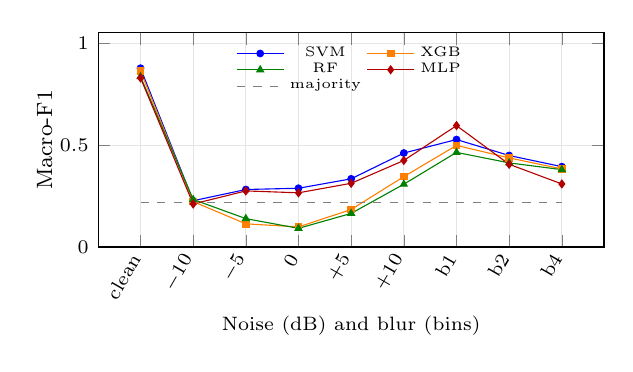
\begin{tikzpicture}
\begin{axis}[
  width=0.66\columnwidth, height=4.3cm,
  ymin=0, ymax=1.05, ylabel={Macro-F1}, ylabel style={font=\footnotesize, yshift=-4pt},
  xtick={0,...,8}, xticklabels={clean,$-10$,$-5$,0,$+5$,$+10$,b1,b2,b4},
  xticklabel style={font=\scriptsize, rotate=60, anchor=east}, yticklabel style={font=\scriptsize},
  legend style={font=\tiny, at={(0.5,0.99)}, anchor=north, legend columns=2, row sep=-3pt, draw=none, fill=none},
  xlabel={Noise (dB) and blur (bins)}, xlabel style={font=\scriptsize, yshift=3pt},
  grid=major, grid style={gray!20}]
\addplot[mark=*, mark size=1.2pt, blue] coordinates {(0,.8771)(1,.2269)(2,.2820)(3,.2882)(4,.3344)(5,.4610)(6,.5272)(7,.4488)(8,.3941)};
\addplot[mark=square*, mark size=1.2pt, orange] coordinates {(0,.8625)(1,.2226)(2,.1136)(3,.0986)(4,.1839)(5,.3453)(6,.4984)(7,.4370)(8,.3830)};
\addplot[mark=triangle*, mark size=1.4pt, green!50!black] coordinates {(0,.8353)(1,.2330)(2,.1392)(3,.0915)(4,.1648)(5,.3080)(6,.4641)(7,.4126)(8,.3795)};
\addplot[mark=diamond*, mark size=1.4pt, red!70!black] coordinates {(0,.8294)(1,.2110)(2,.2751)(3,.2658)(4,.3125)(5,.4244)(6,.5954)(7,.4057)(8,.3093)};
\addplot[dashed, gray, domain=0:8] {0.2183};
\legend{SVM,XGB,RF,MLP,majority}
\end{axis}
\end{tikzpicture}\hspace{-2pt}%
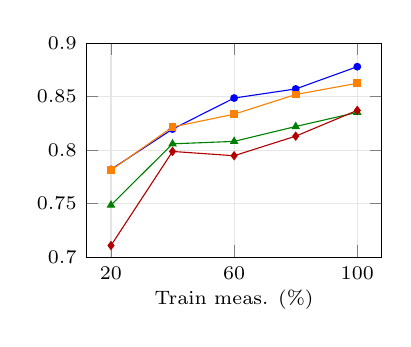
\begin{tikzpicture}
\begin{axis}[
  width=0.44\columnwidth, height=4.3cm,
  ymin=0.70, ymax=0.9, xtick={20,60,100}, ytick={0.7,0.75,0.8,0.85,0.9},
  xlabel={Train meas. (\%)},
  xlabel style={font=\scriptsize, yshift=3pt},
  xticklabel style={font=\scriptsize}, yticklabel style={font=\scriptsize},
  grid=major, grid style={gray!20}]
\addplot[mark=*, mark size=1.2pt, blue] coordinates {(20,.7820)(40,.8197)(60,.8487)(80,.8572)(100,.8780)};
\addplot[mark=square*, mark size=1.2pt, orange] coordinates {(20,.7813)(40,.8217)(60,.8336)(80,.8520)(100,.8625)};
\addplot[mark=triangle*, mark size=1.4pt, green!50!black] coordinates {(20,.7487)(40,.8059)(60,.8082)(80,.8221)(100,.8353)};
\addplot[mark=diamond*, mark size=1.4pt, red!70!black] coordinates {(20,.7109)(40,.7988)(60,.7948)(80,.8131)(100,.8372)};
\end{axis}
\end{tikzpicture}
\caption{Left: macro-F1 under corruption (combined 0\,dB + 2 bins: SVM 0.163, MLP 0.177, XGB 0.072, RF 0.074). Intermediate noise pushes the tree models below the majority baseline. Right: data efficiency for the same four models in the same colours, all still rising at 100\%.}
\label{fig:rob}
\end{figure}

\subsection{Verified LLM reporting (RQ11)}
\emph{Verifier validation.} On seeded summaries containing each of the five error types (unsupported number, altered value, wrong ranking, unsupported comparison, wrong percentage) the verifier detects every error (detection rate 1.00).

\emph{Model study.} Table~\ref{tab:llm} gives the results. Numerical accuracy is at or near 1.000 everywhere: no model fabricated figures at scale. Essentially every failure is a ranking or comparison error, such as naming the wrong model as best on a metric, which a purely numerical check would pass. Constraining the prompt raises the Llama 3.1 8B pass rate from 0.30 to 0.90. The 3B model beats the 8B on the direct arm (15/20 against 6/20, Fisher exact $p=0.010$), but Llama 3.2 is also a later generation, so size and generation cannot be separated. Coverage qualifies the constrained results: the 3B model reports 43 to 47\% of the record, and several of its summaries list all 50 facts, which is transcription rather than summarisation. The correction loop helped once: the 3B model fixed both of its failing generate-and-verify summaries when shown the verifier report (after-fix 1.00), while the 8B model failed to fix its single failure.

\begin{table}[t]
\centering
\caption{LLM reporting: pass rate [Wilson 95\% CI], numerical accuracy, unsupported-claim rate, numbers per summary and coverage.}
\label{tab:llm}
\footnotesize
\setlength{\tabcolsep}{2.6pt}
\begin{tabular}{llccccc}
\toprule
Model & Arm & Pass [CI] & Acc. & Unsup. & Nums & Cov. \\
\midrule
\multirow{3}{*}{\shortstack[l]{Llama 3.1\\8B, $n{=}20$}} & direct & .30 [.15,.52] & .976 & .122 & 7.5 & .15 \\
 & constr. & .90 [.70,.97] & 1.000 & .007 & 12.0 & .24 \\
 & gen+ver. & .95 [.76,.99] & 1.000 & .003 & 12.9 & .26 \\
\midrule
\multirow{3}{*}{\shortstack[l]{Llama 3.2\\3B, $n{=}20$}} & direct & .75 [.53,.89] & 1.000 & .052 & 7.0 & .14 \\
 & constr. & .90 [.70,.97] & .996 & .007 & 21.9 & .43 \\
 & gen+ver. & .90 [.70,.97]$^\dagger$ & .996 & .011 & 23.5 & .47 \\
\midrule
\multirow{3}{*}{\shortstack[l]{Gemini 3.5\\Flash, $n{=}5$}} & direct & 1.00 [.57,1] & & & 15.8 & \\
 & constr. & 1.00 [.57,1] & & & 30.4 & \\
 & gen+ver. & 1.00 [.57,1] & & & 30.8 & \\
\bottomrule
\multicolumn{7}{l}{\scriptsize $^\dagger$ after correction 1.00. Gemini: see text for the partial re-run.}
\end{tabular}
\end{table}

A second Gemini run, stopped by the daily quota, initially gave 3/5 direct; both flags proved to be verifier false positives, discussed below, so that run also stands at 5/5 direct and 5/5 constrained. \emph{Examples.} An accepted summary, Gemini 3.5 Flash, direct arm, 16 numbers, all supported:

\begin{quote}\footnotesize
``The RBF-SVM achieved the highest overall performance, yielding a mean macro F1 of 0.8771 ($\pm$0.0248) and 93.79\% accuracy. XGBoost was highly competitive, achieving a macro F1 of 0.8625 ($\pm$0.0369) and 93.00\% accuracy, while being the most computationally efficient with a training time of 161.4 seconds, over five times faster than SVM (882.5\,s).''
\end{quote}

A rejected summary, Llama 3.2 3B, direct arm, whose numerical factual accuracy is 1.000:

\begin{quote}\footnotesize
``The results showed that the Random Forest (RF) model achieved the highest macro F1 score of 0.8353, followed by XGBoost (XGB) with a score of 0.8625. The Support Vector Machine (SVM) model had the lowest macro F1 score of 0.2183.''
\end{quote}

Every number there is in the record, which is why numerical checking alone accepts it. Two claims are nonetheless false: Random Forest is named best at a value it correctly quotes as below XGBoost's, and 0.2183 is the majority baseline rather than the SVM's score. The verifier reports both as ranking errors. That is the study's central result in one example: faithfulness to the digits does not imply faithfulness to their meaning.

\emph{The verifier is the finding.} Seven bugs were found in the verifier. Six each changed a reported rate, and none was visible from summary metrics. Three of those six were false negatives: an overly broad set of derived values (about 20,000 candidates) could explain an invented macro-F1 as a ratio of two unrelated Brier scores, fixed by pairing only within one metric (282 candidates); direction words such as ``lowest'' were conflated with quality words such as ``best'', inverting checks on losses like ECE; and models were matched in dictionary order rather than sentence order, reversing pairwise comparisons. Three were false positives: sentence-level rather than clause-level binding marked a correct Gemini summary as a ranking error (a spurious pass rate of 0.60); a missing space after a full stop let one clause absorb the next sentence's subject (spurious 0.80); and numbers echoed from the prompt, such as the dwell length, were counted as fabrications, failing all fifteen Llama runs of that version and inverting the study's conclusion. A seventh came from inspecting the two flagged Gemini summaries an interrupted re-run had left unexamined. Both were rejected for the same sentence, ``RBF-SVM and XGBoost offer the best trade-offs between classification accuracy and computational efficiency'', which the clause binder read as a claim that XGBoost has the best accuracy. The subject is conjoined and the superlative ranges over a trade-off between two metrics, so the rejection is a false positive; with it removed, Gemini passes 5 of 5 on the direct arm in both runs. It changed no reported rate, because the affected run was the one we were not reporting, and it surfaced only because a discarded result was inspected rather than dropped. An eighth defect sat in the harness rather than the verifier: one model's results overwrote another's, and filenames now carry the model name. An automatic verifier needs its own validation arm and regression tests (27 now, seven taken from real model output).

\section{Discussion}
\subsection{Answers to the research questions}
\emph{RQ3.} No, and the Atlas run sharpens the answer from a tie to a loss. On these ten descriptors the MLP is the weakest of the four models (0.8294 against 0.8353 for Random Forest and 0.8771 for the SVM) while costing 5.4 times the SVM's training time on better hardware. It earns one genuine point in its favour, which the accuracy table hides: at 0.023\,ms per segment it is the cheapest model to serve, six times faster than XGBoost. That trades 0.033 macro-F1 for a factor of six in latency, so a system bound by inference cost rather than by accuracy could still prefer it. With ten highly redundant inputs and a strong kernel method, there is little nonlinear structure left for a small network to find. \emph{RQ2 (S1 contribution).} The SVM's \pmv{0.8771}{0.0248} is the classical reference against which the S2 to S4 neural models must show gains under identical folds. \emph{RQ9.} No. The most accurate model is the least trustworthy at high confidence: the SVM offers only 3.5\% coverage at $p\ge0.99$ and has the highest confident-error rate. Random Forest is best calibrated by ECE and makes the fewest confident errors, XGBoost has the best Brier score and the most useful confident operating point, and the MLP, despite finishing last on macro-F1 and Brier, still yields 53\% coverage at 99.5\% accuracy. No single model wins on accuracy, calibration and confident coverage together, so the choice depends on which of the three the application needs. A deployment that must act only on confident predictions should prefer XGBoost despite its lower macro-F1. \emph{RQ8.} The SVM degrades most gracefully at every noise level, so under noise the best model is also the most robust, in contrast to RQ9, but not at every condition: the MLP wins at 1-bin blur and in the combined case. All models fail badly under noise. \emph{RQ10 (S1 part).} The decisive descriptors are spectral entropy, Doppler spread and side-lobe energy, which measure how widely energy spreads away from the body line, that is, sidebands and rotor modulation. Zero-Doppler structure matters for hovering drones and reflectors. Periodic temporal signatures contribute little at 15\,ms. \emph{Reproducibility.} Deterministic preprocessing and classical training reproduce exactly across machines while the neural model does not, so a reproducibility claim has to name the hardware. \emph{RQ11.} Current LLMs rarely alter numbers but often misstate rankings; constrained prompting and verification raise pass rates to 0.90 to 0.95, but only if the verifier checks comparisons, and only after the verifier itself has been validated.

\subsection{Positive findings}
Physics-guided descriptors computed from I/Q reach 0.88 macro-F1 and 0.94 accuracy on a measurement-disjoint split with a model that trains in minutes. Results are stable across folds in hyperparameter choice and in which recordings are hard. The error analysis maps cleanly onto physics: speed near the band edge, hovering versus translating flight, running gait and range-dependent SNR. The corruption pipeline is validated by exact reproduction of clean scores, and the LLM study yields a transferable lesson about verification.

\subsection{Negative findings}
The MLP adds nothing here and is in fact last on both macro-F1 and Brier score. The proposed compact subset is poor. The temporal descriptors are nearly useless at this dwell. No model is robust to added noise, and the tree models are worse than guessing at 0\,dB. Part of the reflector decision is learned from range-dependent SNR. The dataset authors' split leaks, so the published benchmark cannot be compared directly. Seven verifier bugs show how easily an automated check can produce confident, wrong conclusions.

\emph{What would make features more robust.} Because the most stable features keep their rank order but shift in scale, a rank or quantile transform fitted on the training fold, or training with noise injected at a range of SNRs, should help markedly. Neither was run, since hyperparameters and preprocessing are frozen; both are natural follow-ups.

\section{Limitations and Pending Work}
Every model chose a value at the edge of its mandated grid ($C=100$, rate 0.1 with depth 6 and 500 trees, lr $10^{-3}$), so all may be under-tuned, a limitation shared by every track. Statistical power rests on 130 measurements rather than 75,801 segments; only 11 human and 19 reflector recordings exist, and the per-fold spread of those two classes (up to 0.118 for humans) is a direct consequence. Peak memory is set by the feature table rather than by the models, so it says nothing about method cost here. The added-noise SNR is relative to recorded power, not true target SNR. Aliasing of rotor tips is inherent to the radar. The Gemini study has $n=5$; Llama generation and size are confounded. The two environments differ in more than one place, scikit-learn 1.9.0 against 1.8.0 and PyTorch 2.13.0 against 2.5.1, so the MLP's cross-machine difference cannot be attributed to the device alone; the classical models are unaffected, and the MLP is reproducible only within one environment. The MLP's batch-one latency comes from a separate job (2308) that loads the stored checkpoints, since the training script does not time inference; same protocol, same node, with a CUDA synchronisation after each inference so the figure is completion rather than launch time.

A second stale-file failure deserves recording, because the report already cites one. The first Atlas attempt (job 2238) died 19 seconds in with argument-parser exit code 2, after staging, preprocessing, feature extraction and the full validation gate had passed: the cluster copy of the training script predated the \texttt{--latency-repeats} option the job script passes. The file checker had called it current, because it tested one behavioural marker string that the older revision also contained. It now requires several markers per file, including the flags the job script passes. Two incidents of the same class say that a checker which is not itself adversarially tested provides false assurance rather than assurance.

Pending: (i) the data-driven compact subset; (ii) feature distributions by class and the correlation matrix as figures. Tables~\ref{tab:main}, \ref{tab:cost} and~\ref{tab:fold} are generated by \texttt{compare\_models.py} from the stored result files and included verbatim, as instruction 13 requires; the remaining numbers in the text are quoted from those same files.

\section{Conclusion}
On physics-guided micro-Doppler descriptors, a calibrated RBF-SVM is the most accurate and most robust of the four S1 models, but not the most trustworthy; XGBoost gives the best confident operating point at a tenth of the inference cost, Random Forest the lowest calibration error, and the MLP finishes last on accuracy and on Brier score while costing the most to train. The descriptors work because they measure how Doppler energy spreads away from the body line. They fail at the zero-Doppler band edge, for hovering and translating drones at opposite tails, at long range, and under any substantial noise. For LLM reporting, numbers are rarely wrong but rankings often are, and a verifier is only as trustworthy as its own tests.

\begin{thebibliography}{99}
\footnotesize
\setlength{\itemsep}{0pt}\setlength{\parskip}{0pt}
\bibitem{karlsson2022} \pending{verify} A. Karlsson, M. Jansson and M. H\"am\"al\"ainen, ``Model-aided drone classification using convolutional neural networks,'' in \emph{Proc. IEEE Radar Conf. (RadarConf22)}, 2022, doi: 10.1109/RadarConf2248738.2022.9764194.
\bibitem{karlsson_zenodo} \pending{verify} A. Karlsson \emph{et al.}, ``Radar measurements of drones, birds, humans and a corner reflector at 77\,GHz,'' Zenodo, 2022, doi: 10.5281/zenodo.5845259.
\bibitem{kumawat2022} H. C. Kumawat, M. Chakraborty, A. A. B. Raj and S. V. Dhavale, ``DIAT-$\mu$SAT: Small aerial targets' micro-Doppler signatures and their classification using CNN,'' \emph{IEEE Geosci. Remote Sens. Lett.}, vol. 19, 2022.
\bibitem{chen2006} V. C. Chen, F. Li, S.-S. Ho and H. Wechsler, ``Micro-Doppler effect in radar: Phenomenon, model, and simulation study,'' \emph{IEEE Trans. Aerosp. Electron. Syst.}, vol. 42, no. 1, pp. 2--21, 2006.
\bibitem{richards} M. A. Richards, \emph{Fundamentals of Radar Signal Processing}, 2nd ed. New York: McGraw-Hill, 2014.
\bibitem{cortes1995} C. Cortes and V. Vapnik, ``Support-vector networks,'' \emph{Mach. Learn.}, vol. 20, pp. 273--297, 1995.
\bibitem{breiman2001} L. Breiman, ``Random forests,'' \emph{Mach. Learn.}, vol. 45, pp. 5--32, 2001.
\bibitem{chen2016} T. Chen and C. Guestrin, ``XGBoost: A scalable tree boosting system,'' in \emph{Proc. ACM SIGKDD}, 2016, pp. 785--794.
\bibitem{platt1999} J. Platt, ``Probabilistic outputs for support vector machines and comparisons to regularized likelihood methods,'' in \emph{Advances in Large Margin Classifiers}, MIT Press, 1999.
\bibitem{guo2017} C. Guo, G. Pleiss, Y. Sun and K. Q. Weinberger, ``On calibration of modern neural networks,'' in \emph{Proc. ICML}, 2017.
\bibitem{brier1950} G. W. Brier, ``Verification of forecasts expressed in terms of probability,'' \emph{Mon. Weather Rev.}, vol. 78, no. 1, pp. 1--3, 1950.
\bibitem{ioffe2015} S. Ioffe and C. Szegedy, ``Batch normalization,'' in \emph{Proc. ICML}, 2015.
\bibitem{srivastava2014} N. Srivastava \emph{et al.}, ``Dropout: A simple way to prevent neural networks from overfitting,'' \emph{J. Mach. Learn. Res.}, vol. 15, pp. 1929--1958, 2014.
\bibitem{loshchilov2019} I. Loshchilov and F. Hutter, ``Decoupled weight decay regularization,'' in \emph{Proc. ICLR}, 2019.
\bibitem{pedregosa2011} F. Pedregosa \emph{et al.}, ``Scikit-learn: Machine learning in Python,'' \emph{J. Mach. Learn. Res.}, vol. 12, pp. 2825--2830, 2011.
\bibitem{paszke2019} A. Paszke \emph{et al.}, ``PyTorch: An imperative style, high-performance deep learning library,'' in \emph{Proc. NeurIPS}, 2019.
\bibitem{wilson1927} E. B. Wilson, ``Probable inference, the law of succession, and statistical inference,'' \emph{J. Amer. Statist. Assoc.}, vol. 22, pp. 209--212, 1927.
\bibitem{ji2023} Z. Ji \emph{et al.}, ``Survey of hallucination in natural language generation,'' \emph{ACM Comput. Surv.}, vol. 55, no. 12, 2023.
\end{thebibliography}

\end{document}
